\chapter{Inorganic Materials and Nanomaterials}\label{ch:b3:inorganic-materials}

A slab of silica \omterm{def:b3:inorganic-materials:sol-gel}{aerogel}, a solid that is mostly air, holds a flower above a gas
flame without letting it wilt. It is a glass, made not by melting sand but by
letting a liquid set into a \omterm{def:b3:colloids:colloid}{gel} and then drying the \omterm{def:b3:colloids:colloid}{gel} without letting it
collapse. Materials chemistry works in that order: choose the structure, then
the route that makes it, then read off the properties. This chapter follows
the routes to inorganic solids, the structures of \omterm{def:b3:inorganic-materials:ceramic}{ceramics}, glasses and porous
crystals, and what happens to matter when a particle is only a few nanometres
across.

\begin{recall}
The Year 1 volume described crystal structure types, interstitial sites,
allotropes, graphite and diamond; the Year 2 volume phase diagrams, the glass
transition temperature and polymers. \Cref{ch:b3:surfaces-catalysis} defined the
\omterm{def:b3:surfaces-catalysis:surface-area}{specific surface area}, \cref{ch:b3:colloids} \omterm{def:b3:colloids:colloid}{sols} and \omterm{def:b3:colloids:colloid}{gels},
\cref{ch:b3:solid-state} bands, \omterm{def:b3:solid-state:defects}{point defects} and \omterm{def:b3:solid-state:ionic-conductor}{ionic conductors};
\cref{ch:b3:quantum-model-systems} solved the \omterm{def:b3:quantum-model-systems:box}{particle in a box}, and
\cref{ch:b3:point-groups} gave the icosahedral group.
\end{recall}

\begin{omfigure}
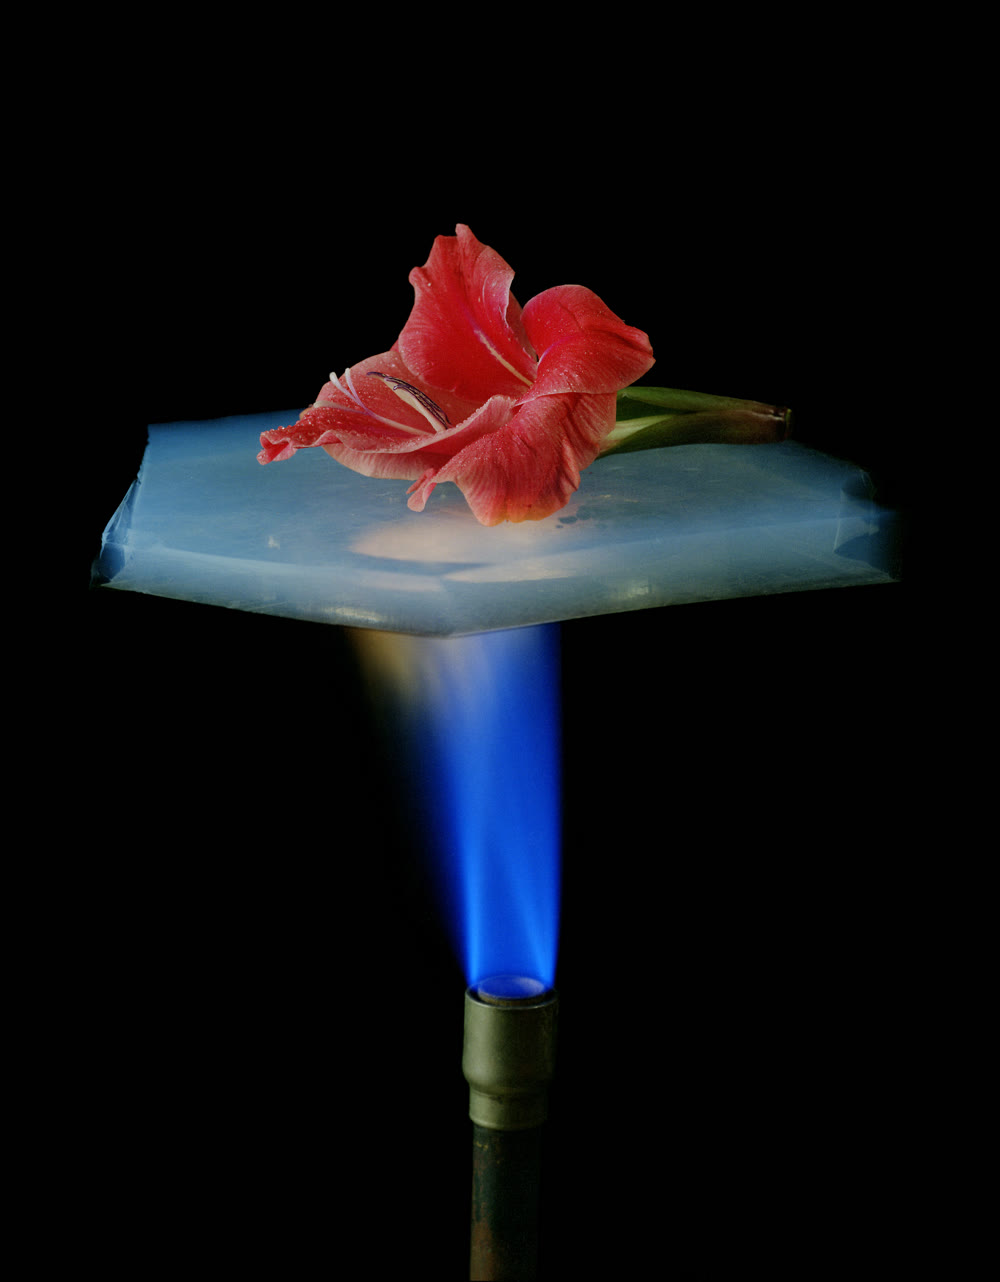
\includegraphics[width=0.38\linewidth]{images/book4/aerogel-flower.jpg}

{\small A flower on a slab of silica \omterm{def:b3:inorganic-materials:sol-gel}{aerogel} above a gas flame: the \omterm{def:b3:inorganic-materials:sol-gel}{aerogel}, a
dried \omterm{def:b3:colloids:colloid}{gel} that is mostly empty space, conducts heat very poorly. Photograph:
NASA/JPL, public domain.}
\end{omfigure}

\section{Synthesis routes}

\begin{definition}[Ceramic method]\label{def:b3:inorganic-materials:ceramic-method}
The \emph{ceramic method}\index{ceramic method} makes a solid compound by
grinding the solid reactants together and heating them, often for days and
with regrinding, at temperatures high enough for ions to diffuse through the
solids.
\end{definition}

The reaction of two solids happens at their contact, and the product forms a
layer between them through which the ions must then travel: the slowest step
is diffusion, and it slows down as the layer thickens.

\begin{proposition}[Parabolic growth]\label{prop:b3:inorganic-materials:parabolic}
If the growth of a product layer is limited by diffusion across it, its
thickness grows as $x^2 = kt$.
\end{proposition}

\begin{proof}
With fixed concentrations on the two faces of the layer, the flux through it
follows Fick's law, $J = D\Delta c/x$. The layer grows in proportion to the flux:
$\dd x/\dd t = \lambda J = \lambda D\Delta c/x$, with $\lambda$ the volume of product per mole transported. Then
$x\,\dd x = \lambda D\Delta c\,\dd t$, and integrating from $x = 0$ at $t = 0$ gives $x^2 = 2\lambda D\Delta c\,t = kt$.
\end{proof}

Doubling the particle size thus multiplies the reaction time by four: hence
fine grinding, mixing at the atomic scale in a precursor (a mixed oxalate or
citrate \omterm{def:b3:colloids:colloid}{gel} that decomposes into the target), or a solution route.

\begin{definition}[Sol--gel process]\label{def:b3:inorganic-materials:sol-gel}
The \emph{sol--gel process}\index{sol--gel process} makes an oxide by
hydrolysis and condensation of molecular precursors, usually alkoxides, in
solution: the solution becomes a \omterm{def:b3:colloids:colloid}{sol} of small oxide clusters, then a \omterm{def:b3:colloids:colloid}{gel}, a
continuous solid network filled with liquid. Dried by evaporation, the \omterm{def:b3:colloids:colloid}{gel}
shrinks into a dense \emph{xerogel}\index{xerogel}; dried above the critical
point of the liquid, which removes it without a liquid--gas interface, it keeps
its volume as an \emph{aerogel}\index{aerogel}.
\end{definition}

\begin{omfigure}
\setchemfig{atom sep=2.0em}
\schemestart
\chemfig{RO-Si(-[2]OR)(-[6]OR)-OR}
\+ \chemfig{H_2O}
\arrow{->[hydrolysis]}[,1.4]
\chemfig{RO-Si(-[2]OR)(-[6]OR)-OH}
\+ ROH
\schemestop
\par\bigskip
\schemestart
\chemfig{{\equiv}Si-OH}
\+
\chemfig{HO-Si{\equiv}}
\arrow{->[condensation]}[,1.6]
\chemfig{{\equiv}Si-O-Si{\equiv}}
\+ \chemfig{H_2O}
\schemestop
\par\medskip

{\small Sol--gel chemistry of a silicon alkoxide (R: an alkyl group, ethyl in
tetraethyl orthosilicate): water replaces alkoxy groups by hydroxy groups, and
two silanols condense into a siloxane bridge. Repeated, the condensations build
a three-dimensional silica network.}
\end{omfigure}

The two reactions together give, for complete reaction,
$\ce{Si(OC2H5)4 + 2H2O -> SiO2 + 4C2H5OH}$. Acid catalysis makes the hydrolysis fast and the
condensation slow, giving thin, chain-like polymers; base catalysis the
opposite, giving dense particles. Coatings (antireflection layers on glass)
are made by dipping a part into the \omterm{def:b3:colloids:colloid}{sol} and drawing it out.

\begin{definition}[Hydrothermal synthesis]\label{def:b3:inorganic-materials:hydrothermal}
\emph{Hydrothermal synthesis}\index{hydrothermal synthesis} crystallises a
solid from water above its normal boiling point, in a closed vessel under its
own vapour pressure; \emph{solvothermal synthesis}\index{solvothermal synthesis}
does the same in another solvent.
\end{definition}

\begin{definition}[Chemical vapour deposition]\label{def:b3:inorganic-materials:cvd}
\emph{Chemical vapour deposition}\index{chemical vapour deposition} (CVD) grows a
solid film on a heated surface by the reaction of gaseous precursors there, as
silicon from silane, $\ce{SiH4 -> Si + 2H2}$, or diamond from methane and hydrogen.
\end{definition}

\begin{method}[Choosing a synthesis route]\label{met:b3:inorganic-materials:route}
\begin{enumerate}
  \item A stable, refractory oxide in bulk powder: the \omterm{def:b3:inorganic-materials:ceramic-method}{ceramic method}, with a
        precursor if mixing is hard.
  \item A metastable phase, a fine powder or a coating at low temperature:
        sol--gel or a precipitation.
  \item Large single crystals of a phase soluble only in hot water (quartz) or
        a framework built around a template (\omterm{def:b3:inorganic-materials:zeolite}{zeolites}): hydrothermal.
  \item A thin, pure film on a substrate (\omterm{def:b3:solid-state:classes}{semiconductor} layers): CVD.
\end{enumerate}
\end{method}

\begin{inthelab}[A sol--gel coating and an autoclave]
Tetraethyl orthosilicate is stirred with ethanol, water and a drop of acid
until the solution is clear; a clean glass slide is dipped in and drawn out at
a steady slow speed, dried and heated, leaving a silica film thin enough to
show interference colours. For a \omterm{def:b3:inorganic-materials:hydrothermal}{hydrothermal synthesis} the reactants are put
in a polytetrafluoroethylene liner, filled no more than about two thirds so
that the expanding liquid does not fill the vessel, sealed in a steel
autoclave and heated in an oven; the autoclave is opened only once cold.
\end{inthelab}

\begin{omfigure}
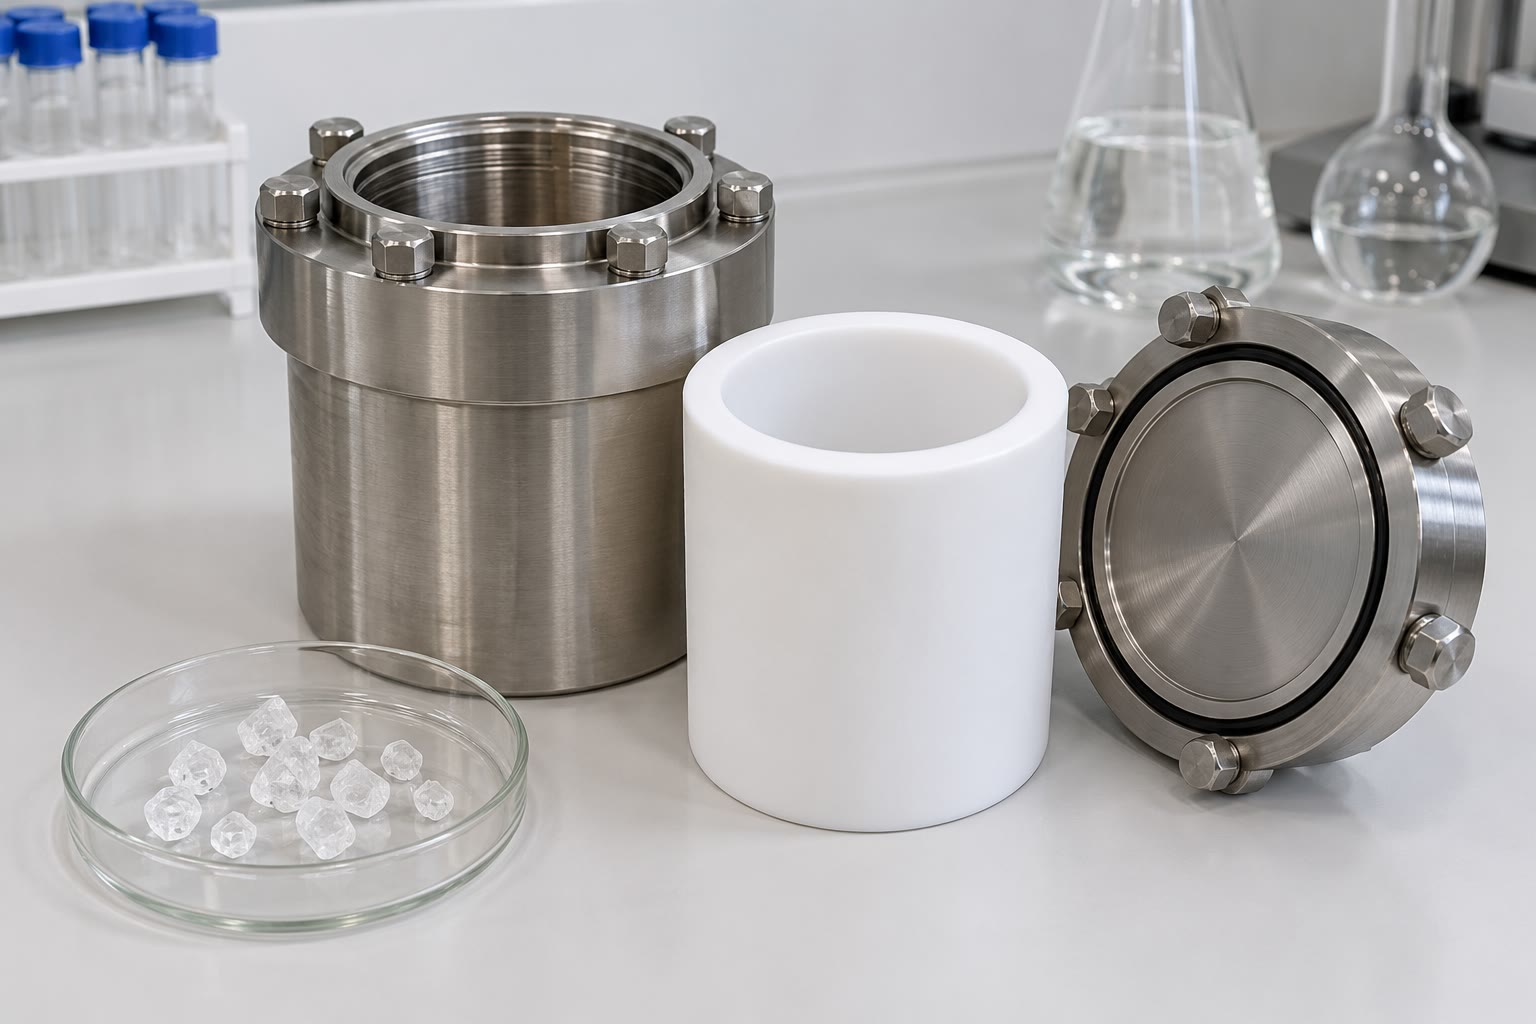
\includegraphics[width=0.5\linewidth]{images/book4/ai/b3-23-autoclave.jpg}

{\small A laboratory autoclave for \omterm{def:b3:inorganic-materials:hydrothermal}{hydrothermal synthesis}: a steel body with a
bolted lid, a white polymer liner that holds the reaction mixture, and crystals
grown in it.}
\end{omfigure}

\section{Ceramics and glasses}

\begin{definition}[Ceramic]\label{def:b3:inorganic-materials:ceramic}
A \emph{ceramic}\index{ceramic} is an inorganic, non-metallic solid made by
heating a powder: oxides, nitrides and carbides, or clay products.
\end{definition}

\begin{definition}[Perovskite structure]\label{def:b3:inorganic-materials:perovskite}
The \emph{perovskite structure}\index{perovskite structure} of an oxide $\mathrm{ABO_3}$
has the small B cations at the centres of corner-sharing $\mathrm{BO_6}$ octahedra and
the large A cations in the twelve-coordinate cavities between them; in the
ideal cubic cell, B is at the centre, O at the face centres, A at the corners.
The \emph{tolerance factor}\index{tolerance factor} measures how well the ions
fit:
\[
  t = \frac{r_A + r_O}{\sqrt2\,(r_B + r_O)}.
\]
\end{definition}

\begin{omfigure}
\tdplotsetmaincoords{60}{100}
\begin{tikzpicture}[tdplot_main_coords, scale=1.5, font=\small,
  aA/.style={om atom, ball color=green!45!black, minimum size=7.4mm},
  aB/.style={om atom, ball color=black!35, minimum size=4.4mm},
  aOs/.style={om atom, ball color=red!80, minimum size=4.8mm}]
  \pic[transform shape] {omcubeo={2}};
  % atoms back to front for view 60/100 (depth 0.853x + 0.150y + 0.5z)
  \node[aA] at (0,0,0) {};
  \node[aA] at (0,2,0) {};
  \node[aOs] (o1) at (0,1,1) {};
  \node[aA] at (0,0,2) {};
  \node[aOs] (o2) at (1,1,0) {};
  \node[aA] at (0,2,2) {};
  \node[aOs] (o3) at (1,0,1) {};
  \node[aB] (b) at (1,1,1) {};
  \node[aOs] (o4) at (1,2,1) {};
  \node[aA] at (2,0,0) {};
  \node[aOs] (o5) at (1,1,2) {};
  \node[aA] at (2,2,0) {};
  \node[aOs] (o6) at (2,1,1) {};
  \node[aA] at (2,0,2) {};
  \node[aA] at (2,2,2) {};
  \begin{scope}[on background layer]
    \draw[omMeth!70, line width=0.6pt] (o1.center) -- (o2.center) -- (o6.center) -- (o5.center) -- cycle
      (o3.center) -- (o2.center) -- (o4.center) -- (o5.center) -- cycle
      (o1.center) -- (o3.center) -- (o6.center) -- (o4.center) -- cycle;
    \draw[bond] (b.center) -- (o1.center) (b.center) -- (o2.center) (b.center) -- (o3.center)
      (b.center) -- (o4.center) (b.center) -- (o5.center) (b.center) -- (o6.center);
  \end{scope}
  \node[anchor=west] at (2,3.35,2) {A};
  \node[anchor=west] at (2,3.35,1) {O};
  \node[anchor=west] at (2,3.35,0) {B};
  \node[aA, minimum size=4mm] at (2,3.2,2) {};
  \node[aOs, minimum size=3.2mm] at (2,3.2,1) {};
  \node[aB, minimum size=3mm] at (2,3.2,0) {};
\end{tikzpicture}

{\small The cubic perovskite cell $\mathrm{ABO_3}$: a B cation (grey) at the centre of an
octahedron of six oxide ions at the face centres (green edges), the A cations
at the corners. Each corner A ion is shared by eight cells and each oxygen by
two: one A, one B and three O per cell.}
\end{omfigure}

\begin{proposition}[Ideal tolerance factor]\label{prop:b3:inorganic-materials:tolerance}
In the ideal cubic perovskite, with the ions touching along the B--O and A--O
directions, $t = 1$.
\end{proposition}

\begin{proof}
With edge $a$, B at the centre and O at a face centre are $a/2$ apart: $r_B + r_O = a/2$.
A at a corner and O at the centre of an adjacent face are half a face diagonal
apart: $r_A + r_O = a\sqrt2/2$. Dividing, $(r_A + r_O)/(r_B + r_O) = \sqrt2$, so $t = 1$.
\end{proof}

When $t$ is slightly below 1, the A ion is too small for its cavity and the
octahedra tilt to close around it, lowering the symmetry; when $t$ is above 1,
the B ion is too small for its octahedron and can move off centre.

\begin{definition}[Ferroelectric]\label{def:b3:inorganic-materials:ferroelectric}
A \emph{ferroelectric}\index{ferroelectric} is a crystal with a spontaneous
electric polarisation that an applied electric field can reverse.
\end{definition}

% ledger: rion:Ba2+XII, rion:Ti4+VI, rion:O2-VI
Barium titanate is the classic case: with $r(\ce{Ba^2+}) = \qty{161}{pm}$ (twelve-coordinate),
$r(\ce{Ti^4+}) = \qty{60.5}{pm}$ and $r(\ce{O^2-}) = \qty{140}{pm}$, $t = 1.06$. Below a transition temperature the
titanium ions shift off centre, all in the same direction within a domain,
and the crystal polarises; the huge permittivity near the transition makes
barium titanate the dielectric of most \omterm{def:b3:inorganic-materials:ceramic}{ceramic} capacitors.

\begin{definition}[Oxide glasses]\label{def:b3:inorganic-materials:glass}
An \emph{oxide glass}\index{oxide glass} is an amorphous oxide solid, made by
cooling a melt without crystallisation. Its \emph{network
formers}\index{network former} ($\ce{SiO2}$, $\ce{B2O3}$, $\ce{P2O5}$) build a continuous network of
corner-sharing polyhedra; its \emph{network modifiers}\index{network modifier}
($\ce{Na2O}$, $\ce{CaO}$) break bridges in that network, each oxide ion added turning one
bridging oxygen into two non-bridging ones, with the cations sitting in the
holes.
\end{definition}

\begin{omfigure}
\begin{tikzpicture}
\begin{axis}[name=c, width=0.5\linewidth, axis equal image, hide axis, xmin=-1.2, xmax=12.6, ymin=-1.2, ymax=8.7]
\addplot[quiver={u=\thisrow{u}, v=\thisrow{v}}, -, black!60, line width=0.6pt] table {figdata/out/bachelor-3-glass-network-crystal-bonds.dat};
\addplot[only marks, mark=*, mark size=2.2pt, omDef] table {figdata/out/bachelor-3-glass-network-crystal-T.dat};
\addplot[only marks, mark=*, mark size=1.3pt, omThm, mark options={fill=white}] table {figdata/out/bachelor-3-glass-network-crystal-O.dat};
\end{axis}
\begin{axis}[at={(c.east)}, anchor=west, xshift=0.2cm, width=0.5\linewidth, axis equal image, hide axis, xmin=-1.2, xmax=12.6, ymin=-1.2, ymax=8.7]
\addplot[quiver={u=\thisrow{u}, v=\thisrow{v}}, -, black!60, line width=0.6pt] table {figdata/out/bachelor-3-glass-network-glass-bonds.dat};
\addplot[only marks, mark=*, mark size=2.2pt, omDef] table {figdata/out/bachelor-3-glass-network-glass-T.dat};
\addplot[only marks, mark=*, mark size=1.3pt, omThm, mark options={fill=white}] table {figdata/out/bachelor-3-glass-network-glass-O.dat};
\addplot[only marks, mark=*, mark size=1.5pt, omThm] table {figdata/out/bachelor-3-glass-network-glass-NBO.dat};
\addplot[only marks, mark=*, mark size=2.6pt, omProp] table {figdata/out/bachelor-3-glass-network-glass-Na.dat};
\end{axis}
\end{tikzpicture}

{\small A two-dimensional picture of a crystal and a glass of the same
composition (blue: three-coordinate formers; open red circles: bridging
oxygens). Left, the crystal repeats one ring. Right, the glass: every former
still has three oxygens at nearly the same distances, but the rings have five,
six or seven members and nothing repeats; at two places a modifier has broken a
bridge, leaving two non-bridging oxygens (filled red) and a cation (orange) in
the hole. Model network, relaxed with springs.}
\end{omfigure}

William Zachariasen argued in 1932 that an oxide forms a glass easily when its
cation is surrounded by few oxygens (three or four), each oxygen links at most
two cations, and the polyhedra share corners, not edges or faces: then a
random network costs little more energy than the crystal. Window glass is
silica with sodium and calcium oxides as modifiers, which lower the melting
temperature. Toughened cover glass for phones is soaked in molten potassium
nitrate: larger $\ce{K+}$ ions replace $\ce{Na+}$ ions in the surface and, being crowded,
put it under compression, so that cracks do not open.

\section{Porous solids: zeolites and frameworks}

\begin{definition}[Zeolites]\label{def:b3:inorganic-materials:zeolite}
A \emph{zeolite}\index{zeolite} is a crystalline aluminosilicate whose
framework of corner-sharing $\ce{SiO4}$ and $\ce{AlO4}$ tetrahedra encloses cages and
channels of molecular size, with exchangeable cations and water inside. A
\emph{molecular sieve}\index{molecular sieve} is a porous solid that admits
molecules according to their size; \emph{shape selectivity}\index{shape selectivity}
is the control of a reaction by the size and shape of the pores in
which it takes place.
\end{definition}

Each $\ce{AlO4}$ tetrahedron carries one negative charge more than an $\ce{SiO4}$
(aluminium(III) in place of silicon(IV)); cations in the cages, $\ce{Na+}$ or $\ce{Ca^2+}$,
balance it, and can be exchanged.

\begin{proposition}[Löwenstein's rule]\label{prop:b3:inorganic-materials:lowenstein}
In a \omterm{def:b3:inorganic-materials:zeolite}{zeolite} framework two $\ce{AlO4}$ tetrahedra never share an oxygen: Al--O--Al links
are absent (an observation on all known aluminosilicate frameworks). As a
consequence the ratio Si/Al of a \omterm{def:b3:inorganic-materials:zeolite}{zeolite} is at least 1.
\end{proposition}

\begin{proof}[Proof of the consequence]
Each aluminium has four oxygens, each shared with a silicon by the rule:
$4N_{\mathrm{Al}}$ Al--O--Si links. Each silicon has only four oxygens, so it takes part in
at most four such links: $4N_{\mathrm{Al}} \le 4N_{\mathrm{Si}}$, that is $N_{\mathrm{Si}}/N_{\mathrm{Al}} \ge 1$. Equality forces every
silicon to have four aluminium neighbours: Si and Al alternate.
\end{proof}

\begin{omfigure}
\tdplotsetmaincoords{55}{135}
\begin{tikzpicture}[tdplot_main_coords, scale=0.85, font=\small, baseline=(current bounding box.center),
  tSi/.style={circle, inner sep=0pt, minimum size=2.6mm, draw=black!70, fill=omDef!80},
  tAl/.style={circle, inner sep=0pt, minimum size=2.6mm, draw=black!70, fill=omProp!80}]
  % edges of a truncated octahedron (vertices: permutations of (0, +-1, +-2));
  % hidden edges (both faces facing away for this view) dashed
  \foreach \a/\b/\c/\d/\e/\f in {-2/-1/0/-2/0/-1, -2/-1/0/-2/0/1, -2/-1/0/-1/-2/0, -2/0/-1/-2/1/0, -2/0/-1/-1/0/-2, -1/-2/0/0/-2/-1, -1/-2/0/0/-2/1, -1/0/-2/0/-1/-2, -1/0/-2/0/1/-2, 0/-2/-1/0/-1/-2, 0/-2/-1/1/-2/0, 0/-1/-2/1/0/-2}
    \draw[black!40, dashed] (\a,\b,\c) -- (\d,\e,\f);
  \foreach \a/\b/\c/\d/\e/\f in {-2/0/1/-2/1/0, -2/0/1/-1/0/2, -2/1/0/-1/2/0, -1/0/2/0/-1/2, -1/0/2/0/1/2, -1/2/0/0/2/-1, -1/2/0/0/2/1, 0/-2/1/0/-1/2, 0/-2/1/1/-2/0, 0/-1/2/1/0/2, 0/1/-2/0/2/-1, 0/1/-2/1/0/-2, 0/1/2/0/2/1, 0/1/2/1/0/2, 0/2/-1/1/2/0, 0/2/1/1/2/0, 1/-2/0/2/-1/0, 1/0/-2/2/0/-1, 1/0/2/2/0/1, 1/2/0/2/1/0, 2/-1/0/2/0/-1, 2/-1/0/2/0/1, 2/0/-1/2/1/0, 2/0/1/2/1/0}
    \draw[black!75, line width=0.7pt] (\a,\b,\c) -- (\d,\e,\f);
  % T atoms back to front; hidden ones paler
  \foreach \x/\y/\z/\k/\v in {-2/-1/0/Si/0, -1/-2/0/Al/0, -2/0/-1/Al/0, 0/-2/-1/Si/0, -1/0/-2/Si/0, 0/-1/-2/Al/0, -2/0/1/Al/1, 0/-2/1/Si/1, -2/1/0/Si/1, 1/-2/0/Al/1, 0/1/-2/Al/1, 1/0/-2/Si/1, -1/0/2/Si/1, 0/-1/2/Al/1, -1/2/0/Al/1, 2/-1/0/Si/1, 0/2/-1/Si/1, 2/0/-1/Al/1, 0/1/2/Al/1, 1/0/2/Si/1, 0/2/1/Si/1, 2/0/1/Al/1, 1/2/0/Al/1, 2/1/0/Si/1}
    \node[t\k, opacity=0.35+0.65*\v] at (\x,\y,\z) {};
\end{tikzpicture}
\hspace{1.2cm}
\begin{tikzpicture}[font=\small, scale=0.8, baseline=(current bounding box.center)]
  \foreach \i in {0,1,2} \foreach \j in {0,1,2} {
    \fill[omDef!70] ($(2.2*\i,2.2*\j)+(-0.28,-0.28)$) rectangle +(0.56,0.56);
  }
  \foreach \i in {0,1} \foreach \j in {0,1,2} {
    \draw[black!70, line width=0.8pt] (2.2*\i+0.28,2.2*\j) -- (2.2*\i+0.75,2.2*\j);
    \draw[black!70, line width=0.8pt] (2.2*\i+1.45,2.2*\j) -- (2.2*\i+1.92,2.2*\j);
    \node[draw=black!70, regular polygon, regular polygon sides=6, minimum size=5.6mm, inner sep=0pt] at (2.2*\i+1.1,2.2*\j) {};
  }
  \foreach \i in {0,1,2} \foreach \j in {0,1} {
    \draw[black!70, line width=0.8pt] (2.2*\i,2.2*\j+0.28) -- (2.2*\i,2.2*\j+0.75);
    \draw[black!70, line width=0.8pt] (2.2*\i,2.2*\j+1.45) -- (2.2*\i,2.2*\j+1.92);
    \node[draw=black!70, regular polygon, regular polygon sides=6, minimum size=5.6mm, inner sep=0pt] at (2.2*\i,2.2*\j+1.1) {};
  }
  \node[font=\scriptsize, align=center] at (1.1,-0.85) {$\ce{Zn4O}$ node $+$ terephthalate linker};
\end{tikzpicture}

{\small Left: a sodalite cage, the building unit of \omterm{def:b3:inorganic-materials:zeolite}{zeolite} A, with a
tetrahedral atom at each corner (oxygens, at the middle of each edge, not
drawn); silicon (blue) and aluminium (orange) alternate, as Löwenstein's rule
requires when Si/Al = 1. Right: a layer of a \omterm{def:b3:inorganic-materials:mof}{metal--organic framework},
schematic: $\ce{Zn4O}$ clusters (squares) joined by benzene-1,4-dicarboxylate
linkers (rings) into a cubic grid with large pores.}
\end{omfigure}

\begin{method}[Formula and exchange capacity of a zeolite]\label{met:b3:inorganic-materials:zeolite-formula}
\begin{enumerate}
  \item Write the framework as $\mathrm{[(AlO_2)_x(SiO_2)_y]^{x-}}$: Si/Al $= y/x$.
  \item The framework charge $-x$ is balanced by cations: $x$ monovalent or $x/2$
        divalent.
  \item The exchange capacity is the amount of exchangeable charge per gram:
        $x/M$ moles of monovalent cations, $x/2M$ of divalent ones, with $M$ the
        molar mass of the formula as weighed (anhydrous or hydrated).
\end{enumerate}
\end{method}

\begin{proposition}[Exchange capacity]\label{prop:b3:inorganic-materials:exchange-capacity}
The capacity of a \omterm{def:b3:inorganic-materials:zeolite}{zeolite} for a cation of charge $z$ is $x/(zM)$ moles per gram,
where $x$ is the number of aluminium atoms in a formula of molar mass $M$.
\end{proposition}

\begin{proof}
Each aluminium contributes one negative charge to the framework; electrical
neutrality requires $x$ units of positive charge, all of them exchangeable, so
$x/z$ cations of charge $z$ per formula unit, that is per mass $M$.
\end{proof}

% ledger: iza:LTA.window, iza:MFI.channels
\omterm{def:b3:inorganic-materials:zeolite}{Zeolite} A has windows of eight tetrahedra, \qty{0.41}{nm} across: water and small
ions pass, branched molecules do not. ZSM-5 has two sets of channels of ten
tetrahedra, about 0.51 to \qty{0.56}{nm}: in the conversion of methanol or the
alkylation of toluene, the slim \textit{para}-xylene diffuses out much faster than
its \textit{ortho} and \textit{meta} isomers, which stay and isomerise. That is \omterm{def:b3:inorganic-materials:zeolite}{shape
selectivity}.

\begin{definition}[Metal--organic frameworks]\label{def:b3:inorganic-materials:mof}
A \emph{metal--organic framework}\index{metal--organic framework} (MOF) is a
crystalline solid built from metal ions or clusters joined by polytopic
organic linkers into a porous network. A \emph{secondary building
unit}\index{secondary building unit} is the metal cluster with its
coordinating groups, treated as one node of the net; \emph{reticular
synthesis}\index{reticular synthesis} is the design of a framework by choosing
nodes and linkers of given geometry so that they assemble into a chosen net.
\end{definition}

% ledger: cod:MOF5.formula, cod:MOF5.a
In MOF-5, $\ce{Zn4O}$ clusters with six carboxylate groups are octahedral nodes,
and benzene-1,4-dicarboxylate linkers join them along the edges of a cubic
net, $a = \qty{25.82}{\angstrom}$ for a cell of eight nodes. Replacing the linker by a longer
one keeps the net and enlarges the pores: that is the reticular idea. Such
frameworks have surface areas of thousands of square metres per gram and are
studied for storing hydrogen and methane and for capturing carbon dioxide.

\begin{definition}[Pore sizes]\label{def:b3:inorganic-materials:pores}
% ledger: pore:micro, pore:macro
By convention, \emph{micropores}\index{micropore} are narrower than \qty{2}{nm},
\emph{mesopores}\index{mesopore} between 2 and \qty{50}{nm}, and
\emph{macropores}\index{macropore} wider than \qty{50}{nm}.
\end{definition}

\omterm{def:b3:inorganic-materials:zeolite}{Zeolites} and most MOFs are microporous; silica \omterm{def:b3:colloids:colloid}{gels} and \omterm{def:b3:inorganic-materials:sol-gel}{aerogels} mesoporous.

\section{Nanoparticles}

\begin{definition}[Nanomaterials]\label{def:b3:inorganic-materials:nano}
A \emph{nanomaterial}\index{nanomaterial} has at least one dimension between
about 1 and \qty{100}{nm}; a \emph{nanoparticle}\index{nanoparticle} has all
three.
\end{definition}

\begin{proposition}[Magic clusters]\label{prop:b3:inorganic-materials:magic}
A cuboctahedral cluster made of a central atom and $n$ complete shells has
\[
  N(n) = \frac{10n^3 + 15n^2 + 11n + 3}{3}
\]
atoms, of which $10n^2 + 2$ are on the surface: 13, 55, 147, 309, \dots
\end{proposition}

\begin{proof}
The $k$-th shell of a cuboctahedron has 12 vertices, 24 edges with $k - 1$ atoms
inside each, 8 triangular faces with $(k - 1)(k - 2)/2$ inner atoms each and 6
square faces with $(k - 1)^2$: in total $12 + 24(k - 1) + 4(k - 1)(k - 2) + 6(k - 1)^2 = 10k^2 + 2$. Then
$N(n) = 1 + \sum_{k=1}^{n}(10k^2 + 2) = 1 + \frac{10n(n + 1)(2n + 1)}{6} + 2n$, which expands to the formula; the
outer shell, $10n^2 + 2$ atoms, is the surface.
\end{proof}

\begin{omfigure}
\begin{tikzpicture}
\begin{axis}[name=a, width=0.47\linewidth, height=5.4cm, xmin=0, xmax=18, ymin=0, ymax=1,
  axis lines=left, xlabel={diameter / \unit{nm}}, ylabel={fraction of atoms on the surface},
  tick label style={font=\scriptsize}, label style={font=\small}]
\addplot[omDef, thick, mark=*, mark size=1pt] table[x=diam_nm, y=fsurf] {figdata/out/bachelor-3-nanoparticle-size.dat};
\end{axis}
\begin{axis}[at={(a.east)}, anchor=west, xshift=1.5cm, width=0.47\linewidth, height=5.4cm,
  xmin=0.8, xmax=6, ymin=0, ymax=3, axis lines=left,
  xlabel={radius $R$ / \unit{nm}}, ylabel={confinement energy / \unit{eV}},
  tick label style={font=\scriptsize}, label style={font=\small}]
\addplot[omThm, thick] table[x=R_nm, y=dE_eV] {figdata/out/bachelor-3-nanoparticle-size-b.dat};
\end{axis}
\end{tikzpicture}

{\small Left: fraction of atoms on the surface of cuboctahedral gold clusters
against their diameter: over half for clusters smaller than about
\qty{3}{nm}, still a fifth at \qty{8}{nm}. Right: confinement energy of an
electron--hole pair in a spherical \omterm{def:b3:inorganic-materials:quantum-dot}{quantum dot} (model \omterm{def:b3:quantum-model-systems:oscillator}{reduced mass} $0.10\,m_e$),
which adds to the \omterm{def:b3:solid-state:band}{band gap} and falls as $1/R^2$.}
\end{omfigure}

With a large fraction of its atoms at the surface, where they have fewer
neighbours, a \omterm{def:b3:inorganic-materials:nano}{nanoparticle} melts at a lower temperature than the bulk metal,
is more reactive, and can be a far better catalyst: bulk gold is inert, gold
particles a few nanometres across oxidise carbon monoxide at room temperature.

\begin{definition}[Quantum dots]\label{def:b3:inorganic-materials:quantum-dot}
A \emph{quantum dot}\index{quantum dot} is a \omterm{def:b3:solid-state:classes}{semiconductor} nanocrystal small
enough that the confinement of its electrons and \omterm{def:b3:solid-state:carriers}{holes} raises its \omterm{def:b3:solid-state:band}{band gap}
above that of the bulk solid.
\end{definition}

\begin{theorem}[Confinement in a sphere]\label{thm:b3:inorganic-materials:quantum-dot}
A particle of mass $m$ confined in a sphere of radius $R$ by infinite walls has
the ground-state energy $E = \hbar^2\pi^2/(2mR^2) = h^2/(8mR^2)$, with wavefunction $\psi \propto \sin(\pi r/R)/r$.
\end{theorem}

\begin{proof}
For a spherically symmetric state $\psi(r) = u(r)/r$, the Laplacian gives
$\nabla^2\psi = u''/r$, so the \omterm{thm:b3:quantum-model-systems:schrodinger}{Schrödinger equation} inside becomes $-\frac{\hbar^2}{2m}u'' = Eu$, that of a particle on a
line. The solution with $\psi$ finite at the centre has $u(0) = 0$: $u = \sin(kr)$, with $E = \hbar^2k^2/2m$.
The wall requires $u(R) = 0$, so $kR = \pi$ for the ground state, and $E = \hbar^2\pi^2/(2mR^2)$.
\end{proof}

In a dot, the electron and the \omterm{def:b3:solid-state:carriers}{hole} are both confined; the energy of the
lowest excitation is $E_g + h^2/(8\mu R^2)$ to a first approximation, with $\mu$ their \omterm{def:b3:quantum-model-systems:oscillator}{reduced
mass} (their Coulomb attraction lowers it a little). Halving the radius
multiplies the confinement energy by four: cadmium selenide dots of a few
nanometres glow red, green or blue according to size alone, and are used as
emitters in displays.

\begin{definition}[Surface plasmon resonance]\label{def:b3:inorganic-materials:plasmon}
A \emph{surface plasmon resonance}\index{surface plasmon resonance} is a
collective oscillation of the conduction electrons of a metal \omterm{def:b3:inorganic-materials:nano}{nanoparticle}
driven by light; it gives a strong absorption band whose wavelength depends on
the metal, the size and shape of the particle and its surroundings.
\end{definition}

Gold \omterm{def:b3:inorganic-materials:nano}{nanoparticles} of a few tens of nanometres absorb green light and look
ruby red in a glass or a \omterm{def:b3:colloids:colloid}{colloid}; as they aggregate, the band shifts to longer
wavelengths and the colour turns blue: the basis of many rapid tests, in which
an antibody-coated gold \omterm{def:b3:colloids:colloid}{colloid} gathers into a coloured line.

\section{Carbon nanomaterials}

\begin{definition}[Carbon nanomaterials]\label{def:b3:inorganic-materials:carbon}
A \emph{fullerene}\index{fullerene} is a closed cage molecule of carbon atoms,
each bonded to three others, with five- and six-membered rings, such as
icosahedral $\ce{C60}$. A \emph{carbon nanotube}\index{carbon nanotube} is a sheet of
graphite rolled into a seamless cylinder about a nanometre across.
\emph{Graphene}\index{graphene} is a single layer of graphite, one atom thick.
\end{definition}

\begin{proposition}[Twelve pentagons]\label{prop:b3:inorganic-materials:euler}
Every \omterm{def:b3:inorganic-materials:carbon}{fullerene} has exactly twelve pentagons, whatever its number of
hexagons.
\end{proposition}

\begin{proof}
A closed cage is a polyhedron: Euler's formula $V - E + F = 2$ holds. Each atom has
three bonds and each bond two atoms: $2E = 3V$. With $p$ pentagons and $h$ hexagons,
counting edges by faces gives $2E = 5p + 6h$, and $F = p + h$. Then $V = 2E/3$ and Euler's
formula reads $-E/3 + p + h = 2$, that is $-(5p + 6h)/6 + p + h = 2$, so $p/6 = 2$: $p = 12$.
\end{proof}

\begin{omfigure}
\begin{tikzpicture}[scale=0.62, font=\small]
  \def\hexd{0.6}
  \begin{scope}
    \clip (-0.4,-0.5) rectangle (9.6,5.2);
    \foreach \i in {-3,...,10} \foreach \j in {-1,...,6} {
      \pgfmathsetmacro\cx{1.7320508*\hexd*(\i + 0.5*\j)}
      \pgfmathsetmacro\cy{1.5*\hexd*\j}
      \draw[black!45] ({\cx+\hexd*cos(30)},{\cy+\hexd*sin(30)})
        \foreach \k in {90,150,...,390} { -- ({\cx+\hexd*cos(\k)},{\cy+\hexd*sin(\k)}) };
    }
  \end{scope}
  \draw[->, thick, omDef] (0,0) -- ({1.7320508*\hexd},0) node[below right, font=\scriptsize, fill=white, inner sep=1pt] {$\mathbf a_1$};
  \draw[->, thick, omDef] (0,0) -- ({1.7320508*\hexd*0.5},{1.5*\hexd}) node[left, font=\scriptsize, fill=white, inner sep=1pt] {$\mathbf a_2$};
  \draw[->, very thick, omThm] (0,0) -- ({1.7320508*\hexd*(4+0.5*2)},{1.5*\hexd*2}) node[above right, font=\scriptsize, fill=white, inner sep=1pt] {$\mathbf C_h = 4\mathbf a_1 + 2\mathbf a_2$};
  \draw[dashed, omMeth, thick] (0,0) -- ({1.7320508*\hexd*9},0) node[right, font=\scriptsize] {zigzag $(n, 0)$};
  \draw[dashed, omProp, thick] (0,0) -- ({1.7320508*\hexd*5*1.5},{1.5*\hexd*5}) node[below right, font=\scriptsize, fill=white, inner sep=1pt] {armchair $(n, n)$};
\end{tikzpicture}

{\small A \omterm{def:b3:inorganic-materials:carbon}{graphene} sheet and the chiral vector of a nanotube: rolling the sheet
so that the tip of $\mathbf C_h = n\mathbf a_1 + m\mathbf a_2$ meets its origin gives the $(n, m)$ tube, here $(4, 2)$.
Along $\mathbf a_1$ the rim of a $(n, 0)$ tube is a zigzag; along $\mathbf a_1 + \mathbf a_2$, at 30°, that of an $(n, n)$
tube is an armchair.}
\end{omfigure}

\begin{proposition}[Metallic and semiconducting nanotubes]\label{prop:b3:inorganic-materials:nanotube}
A single-walled \omterm{def:b3:inorganic-materials:carbon}{carbon nanotube} $(n, m)$ is metallic when $n - m$ is a multiple of 3, and
a \omterm{def:b3:solid-state:classes}{semiconductor} otherwise. \admitted
\end{proposition}

A third of all possible tubes are thus metallic, among them every armchair
tube; the gap of the others falls as their diameter grows. \omterm{def:b3:inorganic-materials:carbon}{Graphene} itself has
no gap at all: its valence and \omterm{def:b3:solid-state:band}{conduction bands} touch at single points, and its
electrons move as if they had no mass.

\begin{safety}{\ghs[0.62cm]{GHS02}\ghs[0.62cm]{GHS07}\ghs[0.62cm]{GHS08}}
% ledger: ghs4:TEOS
Tetraethyl orthosilicate: flammable liquid and vapour, harmful if inhaled,
irritating to the eyes and airways; handled in a fume hood. Nanopowders: the
finest particles reach deep into the lungs, and many are not yet classified;
they are weighed and handled in an enclosure or as a suspension, never as a
loose dust in open air.
\end{safety}

\begin{omfigure}
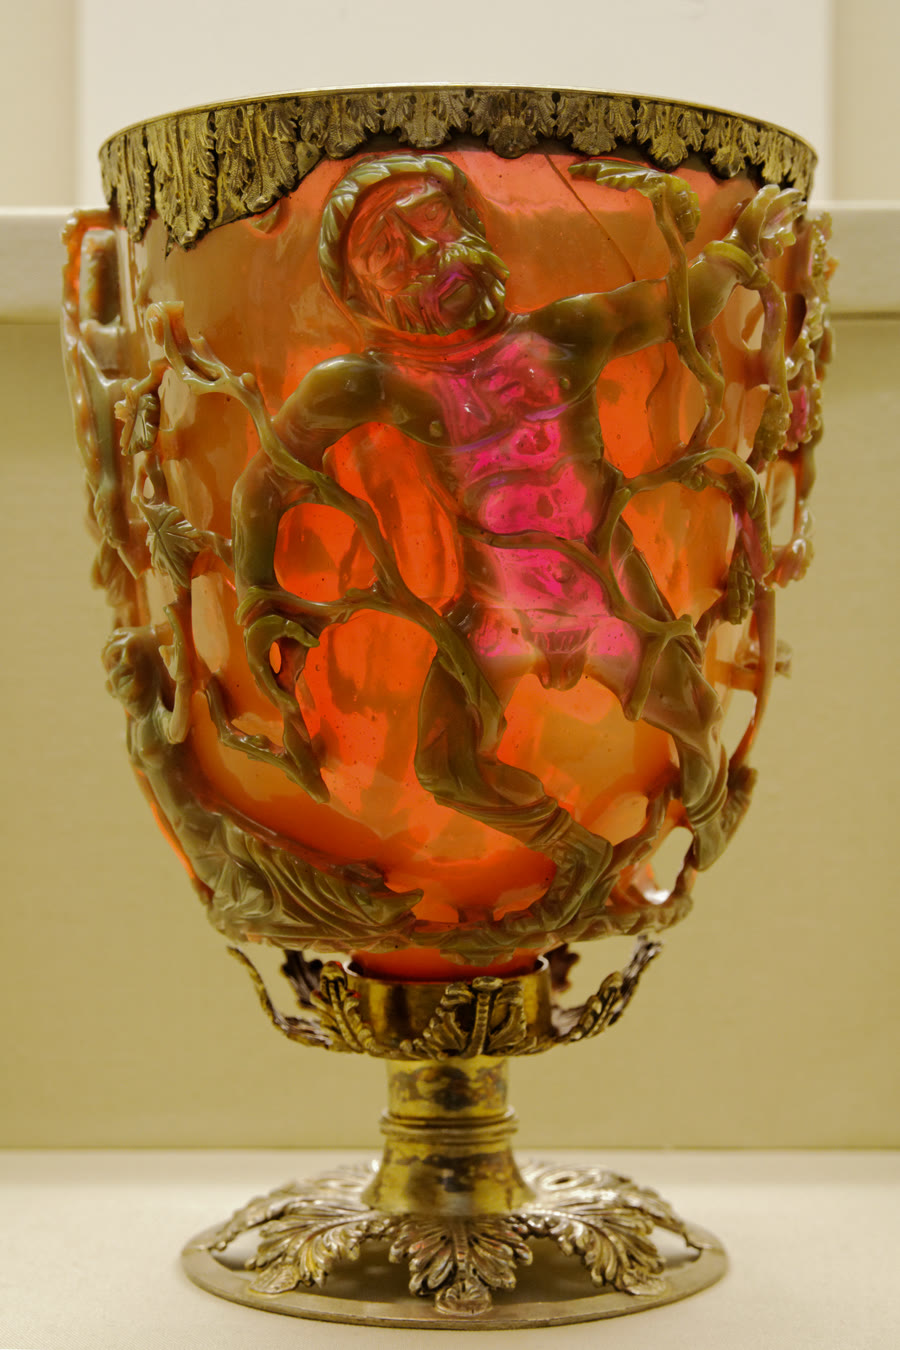
\includegraphics[width=0.32\linewidth]{images/book4/lycurgus-cup.jpg}

{\small The Lycurgus cup, a Roman glass of the fourth century, lit from inside:
it looks green in reflected light and red in transmitted light, an effect of
gold--silver \omterm{def:b3:inorganic-materials:nano}{nanoparticles} in the glass. Photograph: Marie-Lan Nguyen, CC BY
2.5.}
\end{omfigure}

\begin{history}[Nanoparticles before the word, and a football of carbon]
Glassmakers coloured glass red with gold long before anyone knew why; the
Lycurgus cup shows the effect at its most striking. Michael Faraday made gold
\omterm{def:b3:colloids:colloid}{colloids} in the 1850s and saw that their colour came from particles too small
to see. In 1985 Harold Kroto, Robert Curl and Richard Smalley, vaporising
graphite with a laser, found that clusters of sixty carbon atoms were
exceptionally stable and proposed the closed cage of twelve pentagons and
twenty hexagons; they received the 1996 Nobel Prize in Chemistry.
\end{history}

\section{Exercises}

\begin{exercise}[$\star$]\label{exo:b3:inorganic-materials:1}
A product layer between two solids is \qty{2.0}{\micro\metre} thick after \qty{10}{h}. How long until it
is \qty{6.0}{\micro\metre} thick, if the growth is parabolic?
\end{exercise}

\begin{exercise}[$\star$]\label{exo:b3:inorganic-materials:2}
Write the hydrolysis of tetraethyl orthosilicate to silicic acid, the
condensation of two silicic acid molecules, and the overall reaction giving
silica.
\end{exercise}

\begin{exercise}[$\star$]\label{exo:b3:inorganic-materials:3}
Classify $\ce{SiO2}$, $\ce{B2O3}$, $\ce{Na2O}$ and $\ce{CaO}$ as \omterm{def:b3:inorganic-materials:glass}{network formers} or modifiers, and say what
$\ce{Na2O}$ does to the network of silica.
\end{exercise}

\begin{exercise}[$\star$]\label{exo:b3:inorganic-materials:4}
How many pentagons and hexagons does $\ce{C70}$ have? How many bonds?
\end{exercise}

\begin{exercise}[$\star\star$]\label{exo:b3:inorganic-materials:5}
% ledger: rion:Sr2+XII, rion:Ca2+XII, rion:Ba2+XII, rion:Ti4+VI, rion:O2-VI
Compute the \omterm{def:b3:inorganic-materials:perovskite}{tolerance factors} of $\ce{SrTiO3}$, $\ce{BaTiO3}$ and $\ce{CaTiO3}$ with the twelve-coordinate radii
of $\ce{Sr^2+}$ (\qty{144}{pm}), $\ce{Ba^2+}$ (\qty{161}{pm}) and $\ce{Ca^2+}$ (\qty{134}{pm}), $r(\ce{Ti^4+}) = \qty{60.5}{pm}$ and $r(\ce{O^2-}) = \qty{140}{pm}$. What
do they predict?
\end{exercise}

\begin{exercise}[$\star\star$]\label{exo:b3:inorganic-materials:6}
A \omterm{def:b3:inorganic-materials:zeolite}{zeolite} X has the anhydrous formula $\mathrm{Na_{86}[(AlO_2)_{86}(SiO_2)_{106}]}$ (data of the exercise).
Give Si/Al and its exchange capacity for $\ce{Ca^2+}$ in millimoles per gram.
\end{exercise}

\begin{exercise}[$\star\star$]\label{exo:b3:inorganic-materials:7}
% ledger: lat:Au
Gold is face-centred cubic with $a = \qty{407.8}{pm}$. Estimate the number of shells of a
cuboctahedral gold particle about \qty{5}{nm} across, its number of atoms and the
fraction on its surface.
\end{exercise}

\begin{exercise}[$\star\star$]\label{exo:b3:inorganic-materials:8}
A \omterm{def:b3:solid-state:classes}{semiconductor} has a bulk gap of \qty{1.74}{eV}, and its electron and \omterm{def:b3:solid-state:carriers}{hole} a \omterm{def:b3:quantum-model-systems:oscillator}{reduced
mass} of $0.10\,m_e$ (data of the exercise). Estimate the colour of the light emitted by
dots of radius 2.0 and \qty{3.0}{nm}, neglecting the Coulomb attraction.
\end{exercise}

\begin{exercise}[$\star\star$]\label{exo:b3:inorganic-materials:9}
Are the nanotubes $(10, 10)$, $(10, 0)$, $(9, 0)$ and $(12, 8)$ metallic or semiconducting? Which
are armchair, which zigzag?
\end{exercise}

\begin{exercise}[$\star\star\star$]\label{exo:b3:inorganic-materials:10}
% ledger: cod:MOF5.formula, cod:MOF5.a, cod:MOF5.Z
MOF-5, $\mathrm{Zn_4O(C_8H_4O_4)_3}$, is cubic with $a = \qty{25.82}{\angstrom}$ and eight formula units per cell.
Compute its density. If one gram has a surface area of $\qty{3000}{m^2}$ (data of the
exercise), how many football pitches of $\qty{105}{m} \times \qty{68}{m}$ is that?
\end{exercise}

\begin{exercise}[$\star\star\star$]\label{exo:b3:inorganic-materials:11}
Using the shell count of \cref{prop:b3:inorganic-materials:magic}, show that the
surface fraction of a cuboctahedral cluster tends to $3/n$ for large $n$, and
compare with the exact fraction for $n = 8$.
\end{exercise}

\begin{exercise}[$\star\star\star$]\label{exo:b3:inorganic-materials:12}
A closed carbon cage with three bonds per atom contains $p$ pentagons, $h$ hexagons
and $s$ heptagons. Show that $p - s = 12$.
\end{exercise}

\section{Problem: Softening Water with Zeolite A}

\begin{problem}[{Weekend problem --- softening water with zeolite A: the
formula and Löwenstein's rule, the theoretical exchange capacity, the zeolite
needed for one wash, and the window that lets calcium in and keeps detergents
out}]
\label{pb:b3:inorganic-materials:1}
% ledger: iza:LTA.formula, iza:LTA.window, aw:Na, aw:Al, aw:Si, aw:O, aw:H, aw:Ca, aw:C, rion:Ca2+VI
\omterm{def:b3:inorganic-materials:zeolite}{Zeolite} A, used in detergents in place of phosphates, has the formula
$\mathrm{Na_{12}[(AlO_2)_{12}(SiO_2)_{12}]\cdot 27H_2O}$ and windows \qty{0.41}{nm} across. A tap water contains
\qty{2.0}{mmol/L} of $\ce{Ca^2+}$, and a wash uses \qty{15}{L} of it; in the time of a wash the \omterm{def:b3:inorganic-materials:zeolite}{zeolite}
reaches 60\,\% of its capacity (data of the problem).

\medskip\noindent\textbf{Part I --- The formula.}
\begin{enumerate}
  \item Compute the molar mass of the anhydrous formula.
  \item Compute that of the hydrated formula.
  \item Give Si/Al.
  \item State Löwenstein's rule and what it implies here for the arrangement of
        Si and Al.
  \item What is the charge of the framework per formula?
  \item Compute the mass fraction of water in the hydrated \omterm{def:b3:inorganic-materials:zeolite}{zeolite}.
\end{enumerate}

\medskip\noindent\textbf{Part II --- Exchange capacity.}
\begin{enumerate}[resume]
  \item Write the exchange equilibrium between the sodium \omterm{def:b3:inorganic-materials:zeolite}{zeolite} and calcium
        ions.
  \item How many $\ce{Ca^2+}$ can one formula take up?
  \item Compute the theoretical capacity of the anhydrous \omterm{def:b3:inorganic-materials:zeolite}{zeolite} in mmol of $\ce{Ca^2+}$
        per gram.
  \item Compute it for the hydrated \omterm{def:b3:inorganic-materials:zeolite}{zeolite}.
  \item Express the anhydrous capacity as milligrams of $\ce{CaCO3}$ per gram, the usual
        unit for water hardness.
\end{enumerate}

\medskip\noindent\textbf{Part III --- One wash.}
\begin{enumerate}[resume]
  \item Compute the amount of $\ce{Ca^2+}$ in the water of one wash.
  \item Compute the mass of hydrated \omterm{def:b3:inorganic-materials:zeolite}{zeolite} needed at the theoretical capacity.
  \item Compute it at 60\,\% of the capacity.
  \item Compute the mass of sodium released into the water.
  \item Why did detergent makers replace phosphates?
  \item Why does \omterm{def:b3:inorganic-materials:zeolite}{zeolite} A take up $\ce{Mg^2+}$ more slowly than $\ce{Ca^2+}$?
\end{enumerate}

\medskip\noindent\textbf{Part IV --- The window.}
\begin{enumerate}[resume]
  \item Compare the window with the diameter of a $\ce{Ca^2+}$ ion (six-coordinate radius
        \qty{100}{pm}).
  \item What must a hydrated $\ce{Ca^2+}$ ion do to pass?
  \item Why does a \omterm{def:b3:colloids:surfactant}{surfactant} anion such as dodecyl sulfate stay out?
  \item What does \omterm{def:b3:inorganic-materials:zeolite}{zeolite} A do as a drying agent, and why is it called a
        \omterm{def:b3:inorganic-materials:zeolite}{molecular sieve}?
  \item How would replacing $\ce{Na+}$ by $\ce{K+}$ change the size of the molecules admitted?
  \item In ZSM-5, why does \textit{para}-xylene leave the pores faster than \textit{ortho}-xylene?
  \item State the result: the theoretical exchange capacity of anhydrous \omterm{def:b3:inorganic-materials:zeolite}{zeolite} A
        for $\ce{Ca^2+}$.
\end{enumerate}
\end{problem}
